\documentclass[11pt]{beamer}
\usetheme{CambridgeUS}
\usecolortheme{lily}
\usepackage[utf8]{inputenc}
\usepackage{amsmath}
\usepackage{amsfonts}
\usepackage{amssymb}
\usepackage{outlines}
\usepackage{graphicx}
\usepackage{xcolor}
\newcommand{\indep}{\rotatebox[origin=c]{90}{$\models$}}
\usepackage[numbers]{natbib}
\usepackage{pdflscape}
\usepackage{booktabs}
\usepackage{caption}
\usepackage{dcolumn}
\captionsetup{skip=0.333\baselineskip}
\newcolumntype{d}[1]{D{.}{.}{#1}}
\newcommand\mc[1]{\multicolumn{1}{@{}c@{}}{#1}} % handy shortcut macro
\bibliographystyle{acm}
\author{Julio B. Roll \\ Scott Behmer}
\title{Endogenous Heterogeneous Innovation}
%\subtitle{}
\setbeamercovered{transparent} 
\definecolor{brightmaroon}{rgb}{0.76, 0.13, 0.28}
\setbeamercolor{frametitle}{fg=brightmaroon}
\setbeamercolor{title}{fg=brightmaroon}
\setbeamertemplate{navigation symbols}{} 
%\logo{} 
%\institute{} 
\date{March 7, 2018} 
%\subject{} 

\AtBeginSection[]{
  \begin{frame}
  \vfill
  \centering
  \begin{beamercolorbox}[sep=8pt,center,shadow=true,rounded=true]{title}
    \usebeamerfont{title}\insertsectionhead\par%
  \end{beamercolorbox}
  \vfill
  \end{frame}
}

\begin{document}

\begin{frame}
	\maketitle
\end{frame}

\begin{frame}{Theory Outline}
	\begin{itemize}\itemsep12pt
	\item Akcigit and Kerr (2016) included two different types of innovation (incremental and external abrupt). Firms can't do internal abrupt innovation (ex: no internal new product generation) and internal R\&D has no diminishing returns.
	\item We want to endogenize those features. Firms choose how much to invest in internal abrupt or incremental innovations.
	\item We attempt to fit this model to patent citation distributions. The fit gives an impression of how well the model reflects reality. Also, the resulting parameter values have important theoretical interpretations.
	\end{itemize}
\end{frame}

\begin{frame}{Framework - Innovation}
	\textbf{Focus:} Innovation: internal (incremental or abrupt), external, and entrants (the last two only abrupt).
	%my contribution (internal innovation = higher markups)
	\begin{center}
	\begin{figure}\centering\label{Innov5}
	  \fbox{\resizebox{3.2in}{2.2in}{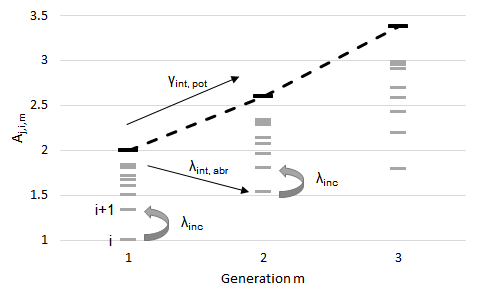
\includegraphics{Innov_5.png}}}
	\end{figure}
	\end{center}
\end{frame}

%The graphics in this slide need to be updated. I want it to have the histogram of abrupt patent citations that we are fitting the model to.
\begin{frame}{Data - Patent Citation Distributions}
	\begin{center}
	\begin{figure}\centering\label{Innov7}
	\begin{minipage}[b]{0.45\linewidth}
	  \fbox{\resizebox{2.0in}{1.8in}{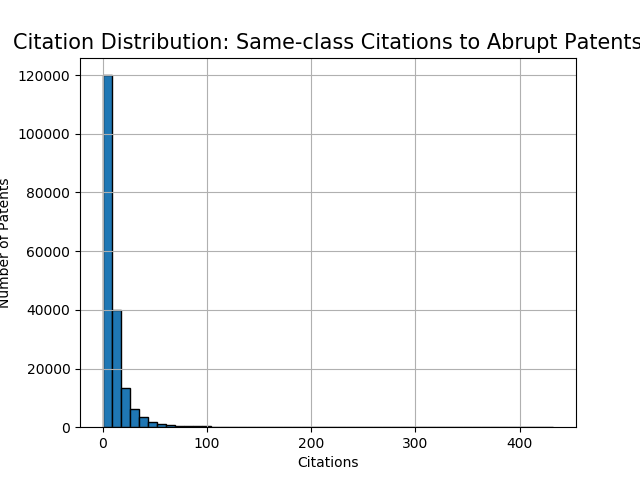
\includegraphics{SameClass_hist.png}}}
	\end{minipage}
	\begin{minipage}[b]{0.45\linewidth}
		\fbox{\resizebox{2.0in}{1.8in}{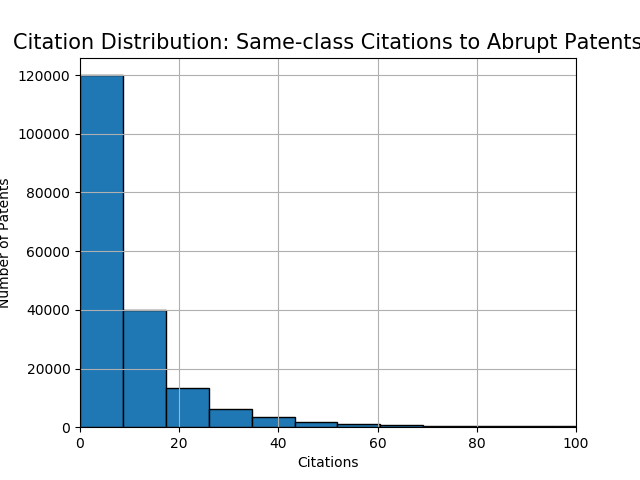
\includegraphics{SameClass_hist_ex0.png}}}
	\end{minipage}
	\end{figure}
	\end{center}
	Summary: \# obs = 189,207; Mean = 10.06; Std. Dev. = 18.43
\end{frame}

\begin{frame}{Theoretical Assumptions Regarding Patent Citations}
	\begin{itemize}\itemsep12pt	
		\item An abrupt patent is cited by every subsequent innovation within its technology cluster.
		\item Technology clusters are all contained within a patent classification.
		\item Abrupt patents will have a large number of citations overall (within and outside of their patent classifications)
		\item We need to choose a cutoff for distinguishing abrupt patents. The default is 10\%. Later we test the robustness of our estimates to changes in this cutoff.
	\end{itemize}
\end{frame}

\begin{frame} {Parameters}
	\begin{itemize}\itemsep 12pt
		\item Three parameters to estimate $\{\alpha , \lambda_{inc, 0}, \lambda_{abr} + \tau \}$
		\item $\alpha$ relates to the diminishing returns of incremental innovations. A low $\alpha$ means that the step-size decreases very quickly. $\alpha = 1$ means that step sizes are constant.
		\item $\lambda_{inc, 0}$ is the rate of incremental innovations for new technology clusters. It is actually a function of the exogenous parameters $\{D, \sigma, \varphi, \xi\}$, which cannot be separated using citation distributions.
%Julio needs to update these other parameters
		\item $\lambda_{abr} + \tau$ is the total arrival rate of abrupt innovations. It is also a function of exogenous parameters.
	\end{itemize}
\end{frame}

\begin{frame} {Estimation Strategy}
	\begin{itemize}\itemsep 12pt
		\item First the parameters $\{\alpha,\frac{\lambda_{inc, 0}}{(\lambda_{abr} + \tau)} \}$ are estimated using MLE on the abrupt, same-class citation distribution.
		\item Next the absolute values of $\lambda_{inc, 0}$ and $\lambda_{abr} + \tau$ are determined using Compustat data on R\&D intensity (= R\&D expenditure/Sales).
	\end{itemize}
\end{frame}

\begin{frame} {Estimation Results}
	\begin{itemize}\itemsep 12pt
		\item $\alpha = 1$, $\lambda_{int, 0}= 0.357 $, $\lambda_{abr} + \tau = 0.0355 $\\
		\begin{center}
		\begin{figure}\centering\label{Innov5}
		  \fbox{\resizebox{3.2in}{2.2in}{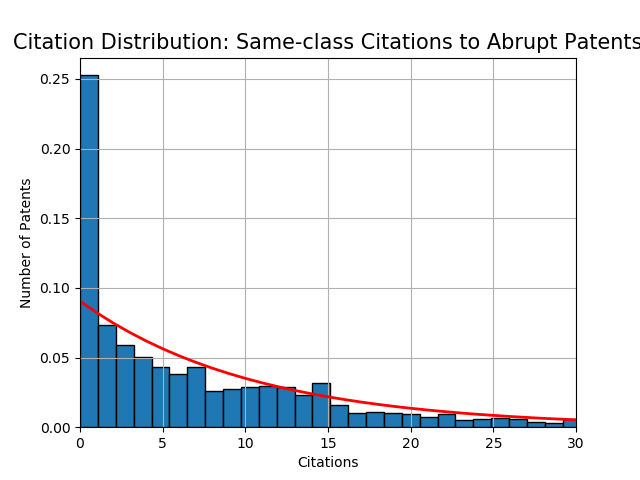
\includegraphics{MLE.png}}}
		\end{figure}
		\end{center}
%Comment on how the alpha estimate implies constant step size. Talk about missing the mass at zero citations.
	\end{itemize}
\end{frame}

\begin{frame} {Confidence in global optimum}
	\begin{itemize}\itemsep 6pt
		\item The result is robust to changes in initial conditions.
		\item "Basin Hopping" confirms the minimum.
		\item We tried fixing $\alpha$ and running an unconstrained optimization. This gave the same results.
		\begin{center}
		\begin{figure}\centering\label{Innov5}
		  \fbox{\resizebox{2.9in}{1.8in}{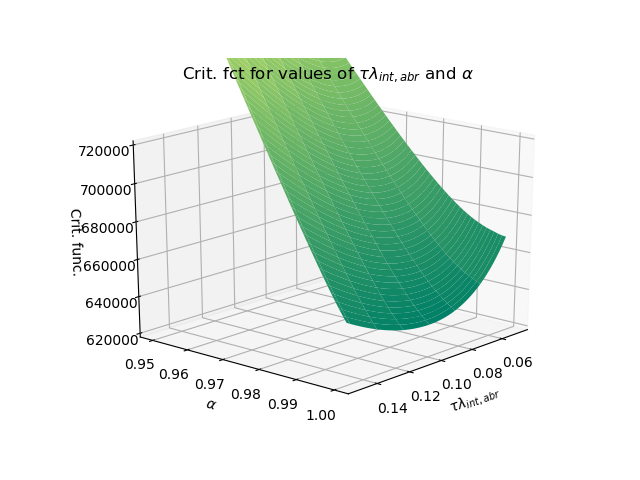
\includegraphics{Crit.png}}}
		\end{figure}
		\end{center}
	\end{itemize}
\end{frame}

\begin{frame} {Robustness}
	\begin{itemize}\itemsep 6pt
		\item We ran a GMM estimation: $\alpha = 1$, $\lambda_{int, 0}= 0.351 $, $\lambda_{abr} + \tau = 0.047 $
		\begin{center}
		\begin{figure}\centering\label{Innov5}
		  \fbox{\resizebox{2.9in}{2.3in}{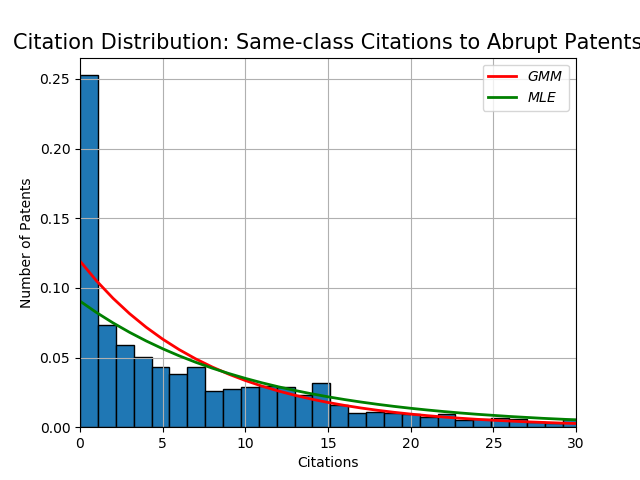
\includegraphics{GMM_MLE.png}}}
		\end{figure}
		\end{center}
	\end{itemize}
\end{frame}

\begin{frame} {Robustness - GMM}
	\begin{itemize}\itemsep 12pt
		\item Moments (GMM):
		\begin{table}
		\centering
		\begin{tabular}{l llp{1.5cm} p{0.5cm} llp{1.5cm}}
		\toprule
		Moment & \multicolumn{1}{c}{Data} & \multicolumn{1}{c}				{Model} \\ 
		\midrule
		Mean of citations & 10.06 & 7.39\\
		Mean of first 5 seq. ratios & 0.57 & 0.88\\
		Sum of first 2 bins & 0.26 & 0.22\\
		R\&D Intensity & 0.068 & 0.068\\
		Criterion & & 0.386\\
		\bottomrule
		\end{tabular}
		\end{table}\vspace{-0.2cm}
		\item Untargeted moment: share of incremental R\&D over total:
		\begin{table}
		\centering
		\begin{tabular}{l llp{1.5cm} p{0.5cm} llp{1.5cm}}
		\toprule
		Moment & \multicolumn{1}{c}{Data} & \multicolumn{1}{c}				{Model} \\ 
		\midrule
		MLE\\
		\;Incremental/total & .90 & .91\\
		GMM\\
		\;Incremental/total & .90 & .88\\
		\bottomrule
		\end{tabular}
		\end{table}
	\end{itemize}
\end{frame}

\begin{frame}{Robustness Results}
	\begin{itemize} \itemsep 12pt
		\item When the cutoff for abrupt patents is adjusted, we get similar results.
	\end{itemize}
	\begin{table}
		\caption*{Robustness Specification Results}
		\centering
		\begin{tabular}{l llp{1.5cm} p{0.5cm} llp{1.5cm}}
			\toprule
			Abrupt Cutoff & \multicolumn{1}{c}{.1} & \multicolumn{1}{c}{.2} & \multicolumn{1}{c}{.05}\\ 
			\midrule
			$\lambda_{inc, 0}$ & .357 & .362 & .347 \\
			$(\lambda_{abr} + \tau)$ & .0355 & .0239 & .0568\\
			$\alpha$ & 1.0 & 1.0 & 1.0\\
			\bottomrule
		\end{tabular}
	\end{table}
\end{frame}

\begin{frame}{Robustness Results}
	\begin{itemize} \itemsep 12pt
		\item We tried relaxing the assumption that abrupt patents are cited by every incremental patent in their technology cluster. Results were identical.
	\end{itemize}
	\begin{table}
		\caption*{Robustness Specification Results}
		\centering
		\begin{tabular}{l llp{1.5cm} p{0.5cm} llp{1.5cm}}
			\toprule
			    & \multicolumn{1}{c}{Baseline} & \multicolumn{1}{c}{Flexible}\\ 
			\midrule
			$\frac{\lambda_{inc, 0}}{(\lambda_{abr} + \tau)}$ & .104 & .104 \\
			$\alpha$ & 1.0 & 1.0\\
			$p$ & - & 1.0 \\
			log-likelihood & -627597 & -627598 \\
			\bottomrule
		\end{tabular}
	\end{table}
\end{frame}

\begin{frame}{Conclusion}
\begin{itemize}\itemsep12pt	
		\item The model fits most of the citation distribution, but badly underestimates the number of  patents with zero citations.
		%discontinuity
		\item No evidence was found for an important feature of the model: the diminishing return from incremental innovations.
		\item We are confident, given our theoretical specification, that we have found the parameters that maximize the log-likelihood.
		\item Our results pass a number of robustness checks.
		\item However, many key theoretical assumptions are still unchecked.
	\end{itemize}
\end{frame}

\begin{frame}{References}
	\nocite{*}
	\bibliography{SE-Proposal}
\end{frame}

\begin{frame}{Appendix: Framework - Innovation}
	\begin{itemize}\itemsep10pt	
	\item Law of motion ($A_{m+1} = A_m\gamma_{int, pot}$): $A_{t+\Delta t} =\begin{cases}
               A_m(1-\alpha^{s})\:,\: \lambda_{inc}\Delta t \:,\: \alpha \in (0,1)\:,\:\ s \in \{1, 2, ...\}\\
               A_t\gamma_{int,abr}\:,\: \lambda_{int,abr}\Delta t\\
               A_t \:, \: \big[1 - \lambda_{inc}\Delta t; 1 - \lambda_{int,abr}\Delta t\big] 
    \end{cases}$
	\item Incremental R\&D cost: $\psi_{inc}(\lambda_{inc}, A_{t}) = \xi_j A_t \lambda_{inc}^{\eta}$
	\item Catching-up: laggards pay $\psi_{inc}(\lambda_{inc}, A_{t})$ and get an arrival $\lambda_{inc} + h$;
	\item Abrupt R\&D cost (for $n_p > 0$): $\psi_{abr}(\lambda_{ext,abr}, \bar{A}_{t}) = \xi_j \bar{A}_t \lambda_{ext,abr}^{\eta}\:$, $\bar{A}_{t}$ sector average;
	%average, to eliminate dependence on R&D level (cst fraction of total expenditure), levels out with returns
	\item Cournot competition: profits $\pi_t$ scale with $\frac{A_{j,i,m}}{\sum_{j}A_{j,i,m}}$ within an industry.
	\end{itemize}
\end{frame}

\begin{frame}{Appendix: Framework - Innovation}
Outside entrepreneur:
	\begin{itemize}\itemsep12pt	
	%present value eq: of max (dividends, returns) discounted with r
	%rP = D + delP/del t: del = capital gains, D dividends
	\item Value function: $rV_0 - \dot{V}_0 = \max\limits_{\lambda_{ext, abr}}\big[\lambda_{ext, abr}\big[E_j\big[V(A_{t, m+1})\big] - V_0\big] - v \bar{A}_{t}\lambda_{ext, abr}\big]$
 	\item Cost: $C_E(\lambda_{ext, abr}, \bar{A}_{t}) = v \bar{A}_{t} \lambda_{ext, abr}\:$, $v$ a constant;
	\item Free entry condition: $E_j\big[V(A_{t, m+1})\big] = v \bar{A}_{t}$
	\item $\Rightarrow$ Each firm faces an aggregate endogenous creative destruction (CD) of rate $\tau_{CE}$ and internal competition rate $\tau_I$.
	\end{itemize}
\end{frame}

\begin{frame}{Appendix: Framework - Innovation}
Incumbents:
	\begin{itemize}
	\item Value function: $rV(A_t) - \dot{V}(A_t) =$\vspace{-3mm} $$ \max_{\substack{\lambda_{inc},\:\lambda_{int, abr}\\\lambda_{ext, abr}}}\left[\begin{aligned}
		&\sum_k^{n_{j, p}}\left[\begin{aligned}
			&\qquad\quad\pi_t n_{j, p} - \{\xi_j\lambda_{inc}^{\eta}A_{t,m};\xi_j\bar{A}_t\lambda_{int, abr}^{\eta}\}\\
			&\ \ + \{\lambda_{inc}\big[V(A_{t,m}^{k-}\cup A_{t+\Delta t,m}^{k}) - V(A_{t,m})\big];\\
			& \lambda_{int, abr}\big[E_j\big[V(A_{t,m}^{k-}\cup A_{t+\Delta t,m+1}^{k}\big] - V(A_{t,m})\big]\}\\
			&\quad\ \ - \tau_I\big[V(A_{t,m}\setminus \bar{A}_{t+\Delta t,m}^{k}) - V(A_{t,m})\big]\\
			&\quad- \tau_{CE}\big[V(A_{t,m}\setminus\bar{A}_{t+\Delta t,m+1}^{k}) - V(A_{t,m})\big]
		\end{aligned}\right]\\
		&\quad+ \lambda_{ext, abr}\big[E_j\big[V(A_{t,m}^{k}\cup A_{t+\Delta t,m+1}^{k'}\big] - V(A_{t,m})\big]\\
		&\qquad\qquad\qquad\quad- \xi_j\bar{A}_t\lambda_{int, abr}^{\eta} - \Phi\bar{A}_t
	\end{aligned}\right]$$
	\end{itemize}
	\vspace{-3mm}
	\begin{columns}
	\begin{column}{0.5\textwidth}
	\begin{itemize}\itemsep3pt	
   	\item 1\textsuperscript{st}: instant returns - costs;
	\item 2\textsuperscript{nd}, 3\textsuperscript{rd}: return from int. R\&D;
	\item 4\textsuperscript{th}: internal competition;
	\end{itemize}
	\end{column}
	\begin{column}{0.5\textwidth}
	\begin{itemize}\itemsep3pt	
	\item 5\textsuperscript{th}: external CE;
	\item 6\textsuperscript{th}: return from abr. R\&D;
	\item 7\textsuperscript{th}: Abr. R\&D and fixed costs;
	\end{itemize}    
	\end{column}
	\end{columns}			
\end{frame}

\end{document}